\documentclass[final]{beamer}

% ====================
% Packages
% ====================

\usepackage[T1]{fontenc}
\usepackage{lmodern}
\usepackage[orientation=landscape,size=a0,scale=1.0]{beamerposter}
\usetheme{confposter}
\usecolortheme{cripac}
\usepackage{graphicx}
\usepackage{booktabs}
%\usepackage{outlines}
\usepackage{amsmath,amssymb,amsfonts}
\usepackage{multirow}
\usepackage[export]{adjustbox}
\usepackage{colortbl}
\usepackage{xcolor}
\usepackage{tikz}
\usetikzlibrary{calc,positioning}

\definecolor{sgreen}{HTML}{27AE60}
\definecolor{hlgreen}{HTML}{E8F8F0}
\definecolor{keyblue}{HTML}{2980B9}
\definecolor{lightbg}{HTML}{F0F4F8}
\definecolor{emphred}{HTML}{E74C3C}

\newcommand{\sUp}[1]{{\color{sgreen}\textbf{#1}}}

% ====================
% Lengths — 3 columns
% ====================

\newlength{\sepwidth}
\newlength{\colwidth}
\setlength{\sepwidth}{0.02\paperwidth}
\setlength{\colwidth}{0.3\paperwidth}

\newcommand{\separatorcolumn}{\begin{column}{\sepwidth}\end{column}}

\usepackage[tableposition=bottom]{caption}
\captionsetup[table]{skip=6pt}
\captionsetup[figure]{skip=6pt}

% ====================
% Metadata
% ====================

\title{Predict the Retrieval! Test Time Adaptation for\\Retrieval Augmented Generation}

\author{Xin Sun$^{1,2,3}$ \enspace Zhongqi Chen$^{1,2}$ \enspace Qiang Liu$^{1,2}$ \enspace Shu Wu$^{1,2}$ \enspace Bowen Song$^{3}$ \enspace Weiqiang Wang$^{3}$ \enspace Zilei Wang$^{*}$ \enspace Liang Wang$^{1,2}$}

\institute[shortinst]{$^1$CRIPAC, Institute of Automation, CAS \samelineand $^2$UCAS \samelineand $^3$Ant Group \samelineand $^*$USTC}

\setconferencename{IEEE International Conference on Acoustics, Speech, and Signal Processing (ICASSP 2026)}
\setmail{xin.sun@cripac.ia.ac.cn}
\setlogo{logo.png}

% ====================
% Body
% ====================

\begin{document}

\begin{frame}[t]

\begin{columns}[t]
\separatorcolumn

% ============================================================
% COLUMN 1: Introduction + Method Overview
% ============================================================
\begin{column}{\colwidth}

  \begin{block}{Introduction \& Motivation}

  \heading{Background}
  \begin{itemize}
    \item\textbf{Retrieval-Augmented Generation (RAG)} enhances LLMs by integrating external knowledge, improving accuracy and reducing hallucinations.
    \itemHowever, RAG systems face significant \textbf{distribution shift} challenges in \textbf{specialized domains} (e.g., finance, medicine), leading to suboptimal generalization.
  \end{itemize}

  \heading{Key Idea}
  \begin{itemize}
    \item\textbf{Test-time adaptation (TTA)} allows models to dynamically adjust parameters at inference time using self-supervised objectives --- \textbf{no labeled data required}.
    \itemWe propose \textbf{TTARAG}: splitting retrieved passages into \textbf{prefix-suffix pairs} and training the model to predict suffix from prefix as a self-supervised signal for domain adaptation.
  \end{itemize}

  \end{block}

  \begin{block}{Method: TTARAG}

  \begin{figure}
    \centering
    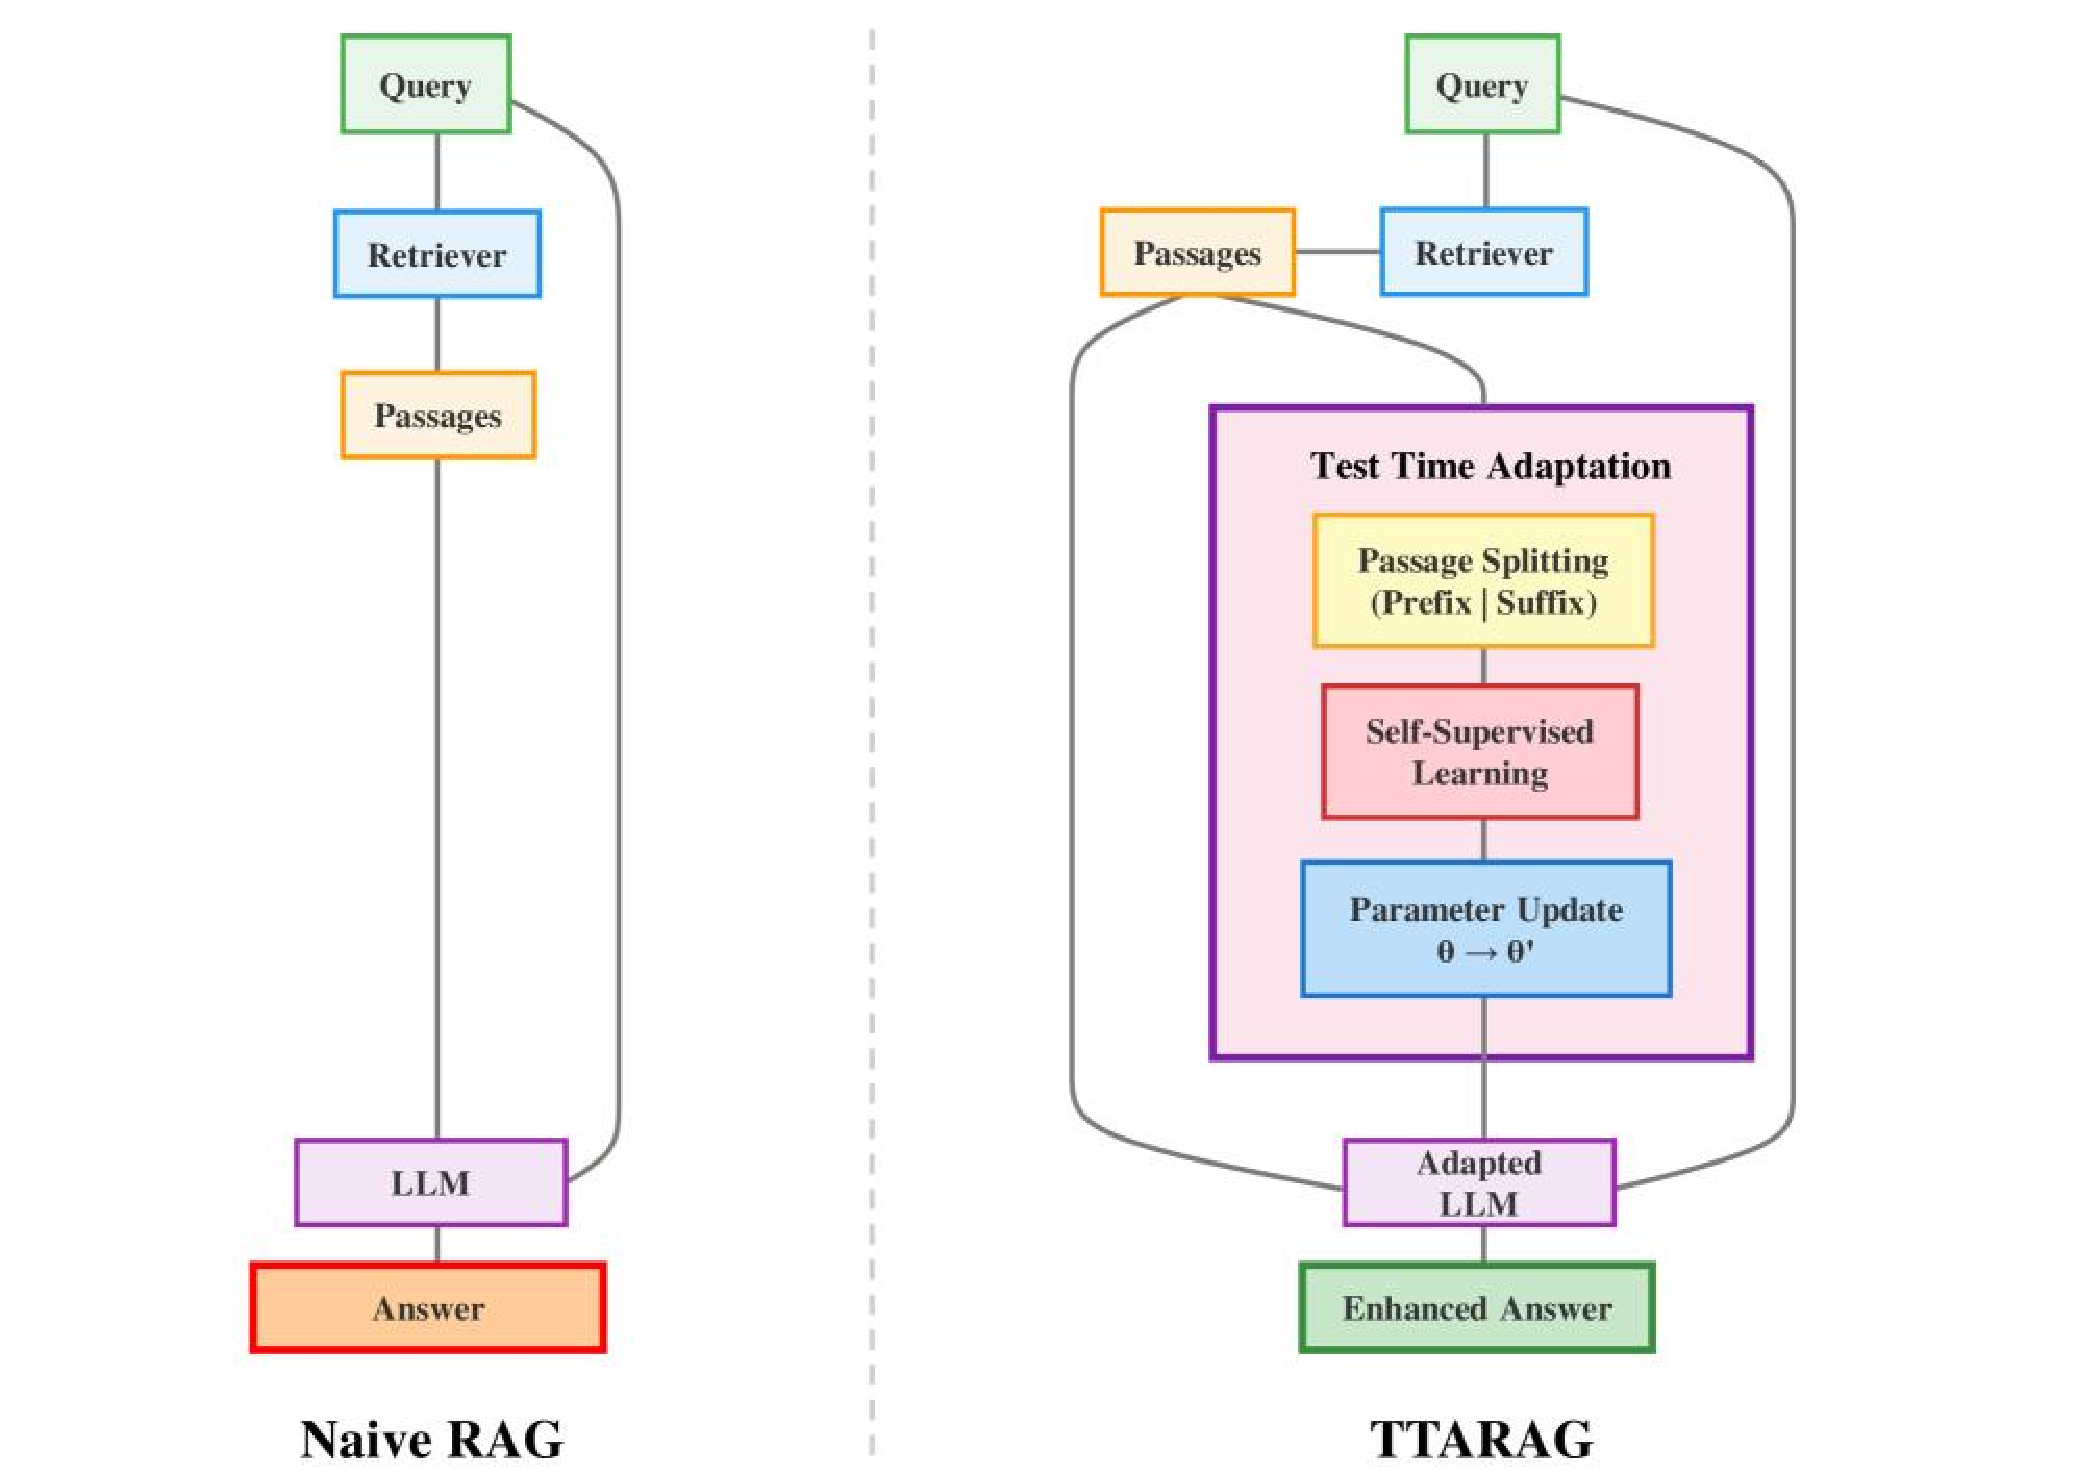
\includegraphics[width=0.88\linewidth]{figures/framework.pdf}
    \caption{Standard RAG vs. TTARAG: our method adds a test-time adaptation module that splits passages, performs self-supervised learning, and updates parameters before answering.}
  \end{figure}

  \end{block}

  \begin{alertblock}{Key Contributions}

  \begin{itemize}
    \itemA \textbf{simple yet effective} test-time adaptation method for RAG via prefix-suffix self-supervised learning.
    \item\textbf{No labeled data} required --- only retrieved passages are used.
    \item\textbf{Consistent improvements} across 6 specialized domains with 3 different LLM backbones.
    \item\textbf{Computationally efficient}: 2.45s vs 4.32s/query (CoT).
  \end{itemize}

  \end{alertblock}

\end{column}

\separatorcolumn

% ============================================================
% COLUMN 2: Technical Details
% ============================================================
\begin{column}{\colwidth}

  \begin{block}{Technical Details}

  \heading{Step 1: Context Processing \& Passage Splitting}
  \begin{itemize}
    \itemFilter out passages below a minimum length threshold to ensure sufficient context.
    \itemSplit each passage into prefix-suffix pairs:
    \begin{itemize}
      \2 \textbf{Primary:} Split at natural linguistic boundaries (periods, commas, semicolons).
      \2 \textbf{Fallback:} Divide at the midpoint when no punctuation split exists.
    \end{itemize}
  \end{itemize}

  \heading{Step 2: Self-Supervised Adaptation}

  Given a query $q$ and retrieved passages $\{p_1, \ldots, p_k\}$, we define the \textbf{self-supervised adaptation loss}:

  \begin{equation}
    \boxed{\mathcal{L}_{adapt} = -\sum_{i=1}^{k} \log P\!\left(p_i^{\text{suffix}} \mid p_i^{\text{prefix}}, q;\, \theta\right)}
  \end{equation}

  The model learns to predict the suffix of retrieved documents from their prefix, aligning its representations with domain-specific language patterns.

  \heading{Step 3: Parameter Update}

  Model parameters are updated via gradient descent with accumulation:

  \begin{equation}
    \theta_t = \theta_{t-1} - \alpha \cdot \frac{1}{N}\sum_{i=1}^{N} \nabla_\theta \mathcal{L}_{adapt}^{i}
  \end{equation}

  After adaptation, generate the final response with updated parameters $\theta'$:

  \begin{equation}
    y = \arg\max_y \; P\!\left(y \mid q, \{p_1, \ldots, p_k\};\, \theta'\right)
  \end{equation}

  \end{block}

  \begin{block}{Ablation Study}

  \heading{Segmentation Strategy}

  \begin{table}
    \centering
    \begin{tabular}{l|ccc}
      \toprule
      \textbf{Strategy} & \textbf{Llama-3.1-8B} & \textbf{Llama-2-7B} & \textbf{ChatGLM-6B} \\
      \midrule
      \textbf{TTARAG} & \textbf{31.9} & \textbf{30.5} & \textbf{25.7} \\
      w/o segmentation & 30.8 & 30.1 & 25.0 \\
      \midrule
      $\Delta$ & \sUp{+1.1} & \sUp{+0.4} & \sUp{+0.7} \\
      \bottomrule
    \end{tabular}
    \caption{Prefix-suffix segmentation consistently outperforms full-passage next-token prediction across all backbones.}
  \end{table}

  \heading{Computation Efficiency}

  \begin{table}
    \centering
    \begin{tabular}{l|ccc|c|c}
      \toprule
      & \textbf{1 pair} & \textbf{3 pairs} & \textbf{5 pairs} & \textbf{CoT} & \textbf{Naive-RAG} \\
      \midrule
      Avg (s/query) & 1.75 & 2.45 & 2.60 & 4.32 & 0.36 \\
      \bottomrule
    \end{tabular}
    \caption{TTARAG is $\sim$\textbf{1.8$\times$ faster} than CoT while achieving better accuracy.}
  \end{table}

  \end{block}

\end{column}

\separatorcolumn

% ============================================================
% COLUMN 3: Results + Analysis
% ============================================================
\begin{column}{\colwidth}

  \begin{block}{Main Results}

  \begin{table}
    \centering
    \resizebox{\linewidth}{!}{
    \begin{tabular}{ll|cccccc|cc}
      \toprule
      & & \multicolumn{6}{c|}{\textbf{CRAG Benchmark}} & \multicolumn{2}{c}{\textbf{Medical}} \\
      \cmidrule(lr){3-8} \cmidrule(lr){9-10}
      \textbf{Backbone} & \textbf{Method} & Finance & Sports & Music & Movie & Open & Overall & BioASQ & PubMed \\
      \midrule
      \multirow{3}{*}{\shortstack[l]{Llama-3.1\\8B-it}}
      & Naive-RAG & 17.4 & 27.6 & 34.9 & 31.3 & 42.4 & 29.8 & 55.6 & 46.6 \\
      & +CoT & 17.9 & 30.2 & 37.6 & 31.5 & \textbf{45.8} & 31.6 & 54.6 & 50.8 \\
      \rowcolor{hlgreen}
      & \textbf{TTARAG} & \textbf{20.1} & \textbf{29.5} & \textbf{37.7} & \textbf{34.6} & 41.5 & \textbf{31.9} & \textbf{75.0} & \textbf{57.4} \\
      \midrule
      \multirow{3}{*}{\shortstack[l]{Llama-2\\7B-chat}}
      & Naive-RAG & 14.7 & 23.2 & 36.5 & 30.4 & 39.2 & 27.8 & 54.1 & 47.6 \\
      & +CoT & 15.7 & 26.7 & 34.3 & 31.4 & \textbf{41.5} & 29.1 & 55.1 & 48.2 \\
      \rowcolor{hlgreen}
      & \textbf{TTARAG} & \textbf{16.4} & \textbf{25.8} & \textbf{40.7} & \textbf{33.8} & 41.1 & \textbf{30.5} & \textbf{71.8} & \textbf{54.0} \\
      \midrule
      \multirow{3}{*}{\shortstack[l]{ChatGLM\\3-6B}}
      & Naive-RAG & 9.8 & 18.7 & 31.4 & 22.4 & 33.4 & 22.0 & 51.4 & 19.8 \\
      & +CoT & 12.7 & 20.6 & 28.4 & 25.8 & 33.9 & 23.6 & 44.3 & 22.4 \\
      \rowcolor{hlgreen}
      & \textbf{TTARAG} & \textbf{14.0} & \textbf{22.1} & \textbf{33.5} & \textbf{25.5} & \textbf{38.1} & \textbf{25.7} & \textbf{58.4} & \textbf{44.8} \\
      \bottomrule
    \end{tabular}
    }
    \caption{Accuracy (\%) across domains. TTARAG achieves consistent improvements, with strong gains in medical domains (\sUp{+19.4\%} BioASQ, \sUp{+25.0\%} PubMedQA).}
  \end{table}

  \heading{vs. Pretrained RAG Models (Llama-2-7B)}

  \begin{table}
    \centering
    \resizebox{\linewidth}{!}{
    \begin{tabular}{l|cccccc|cc}
      \toprule
      \textbf{Model} & Finance & Sports & Music & Movie & Open & Overall & BioASQ & PubMed \\
      \midrule
      Ret-Robust & 14.6 & 20.6 & 33.2 & 32.4 & 33.5 & 26.1 & 24.7 & 28.4 \\
      RAAT & 13.4 & 18.1 & 28.6 & 25.2 & 31.7 & 22.7 & 64.9 & 46.6 \\
      Self-RAG & 11.4 & 19.8 & 22.5 & 20.9 & 26.7 & 19.8 & 57.1 & 43.4 \\
      \rowcolor{hlgreen}
      \textbf{TTARAG} & \textbf{16.4} & \textbf{25.8} & \textbf{40.7} & \textbf{33.8} & \textbf{41.1} & \textbf{30.5} & \textbf{71.8} & \textbf{54.0} \\
      \bottomrule
    \end{tabular}
    }
    \caption{TTARAG outperforms all pretrained RAG models across \textbf{all domains} without task-specific fine-tuning.}
  \end{table}

  \end{block}

  \begin{block}{Hyperparameter Analysis}

  \begin{minipage}[t]{0.48\linewidth}
    \begin{figure}
      \centering
      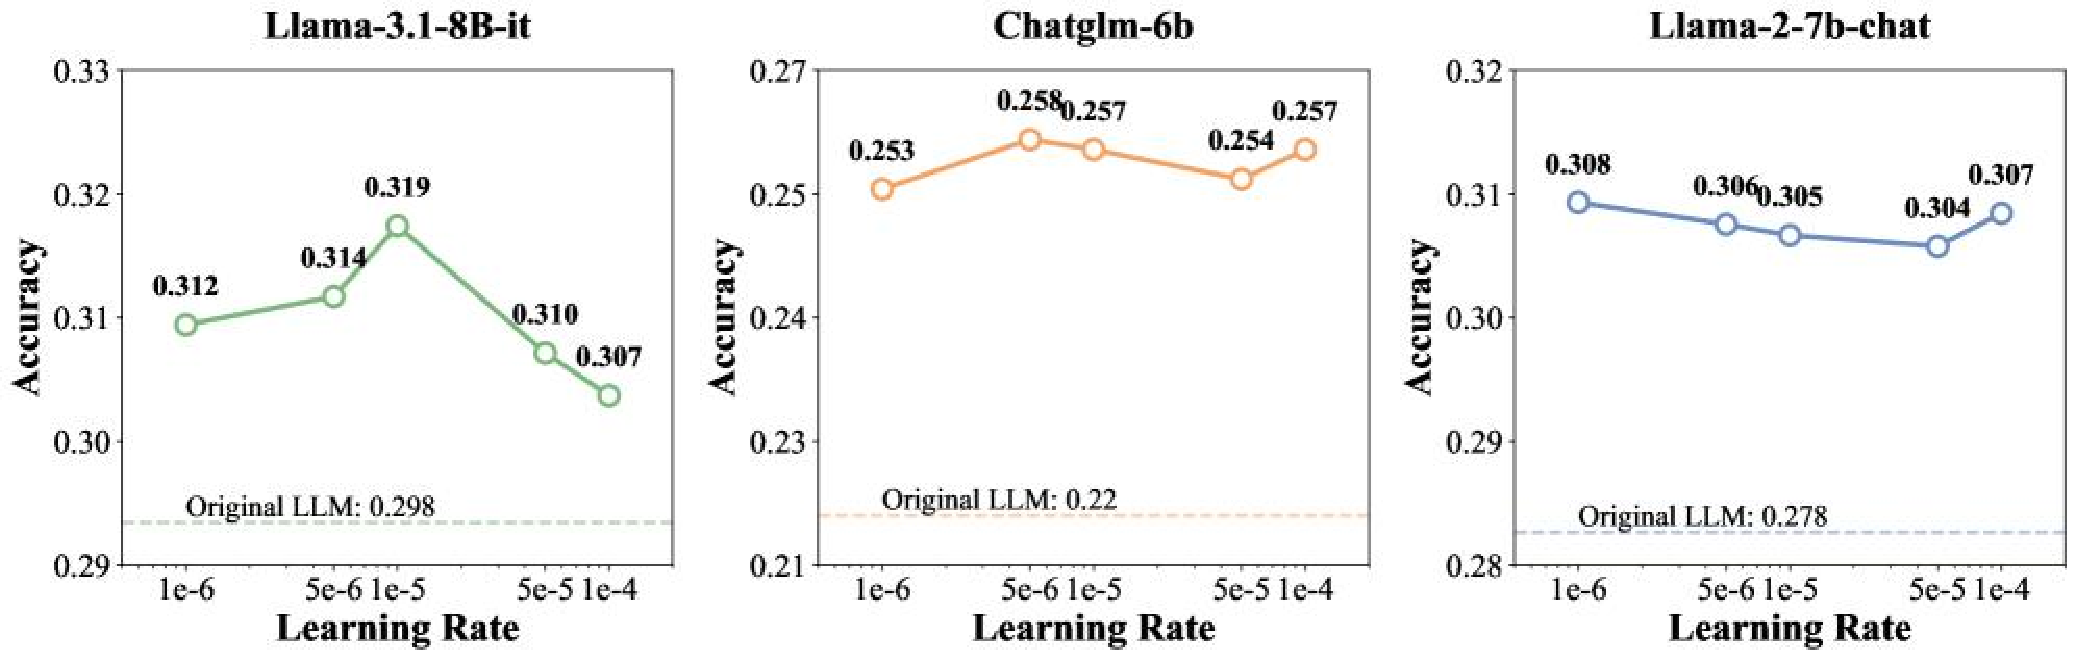
\includegraphics[width=0.95\linewidth]{figures/lr_analysis.pdf}
      \caption{Accuracy vs. Learning Rate. LR $\in [10^{-6}, 10^{-5}]$ is optimal.}
    \end{figure}
  \end{minipage}
  \hfill
  \begin{minipage}[t]{0.48\linewidth}
    \begin{figure}
      \centering
      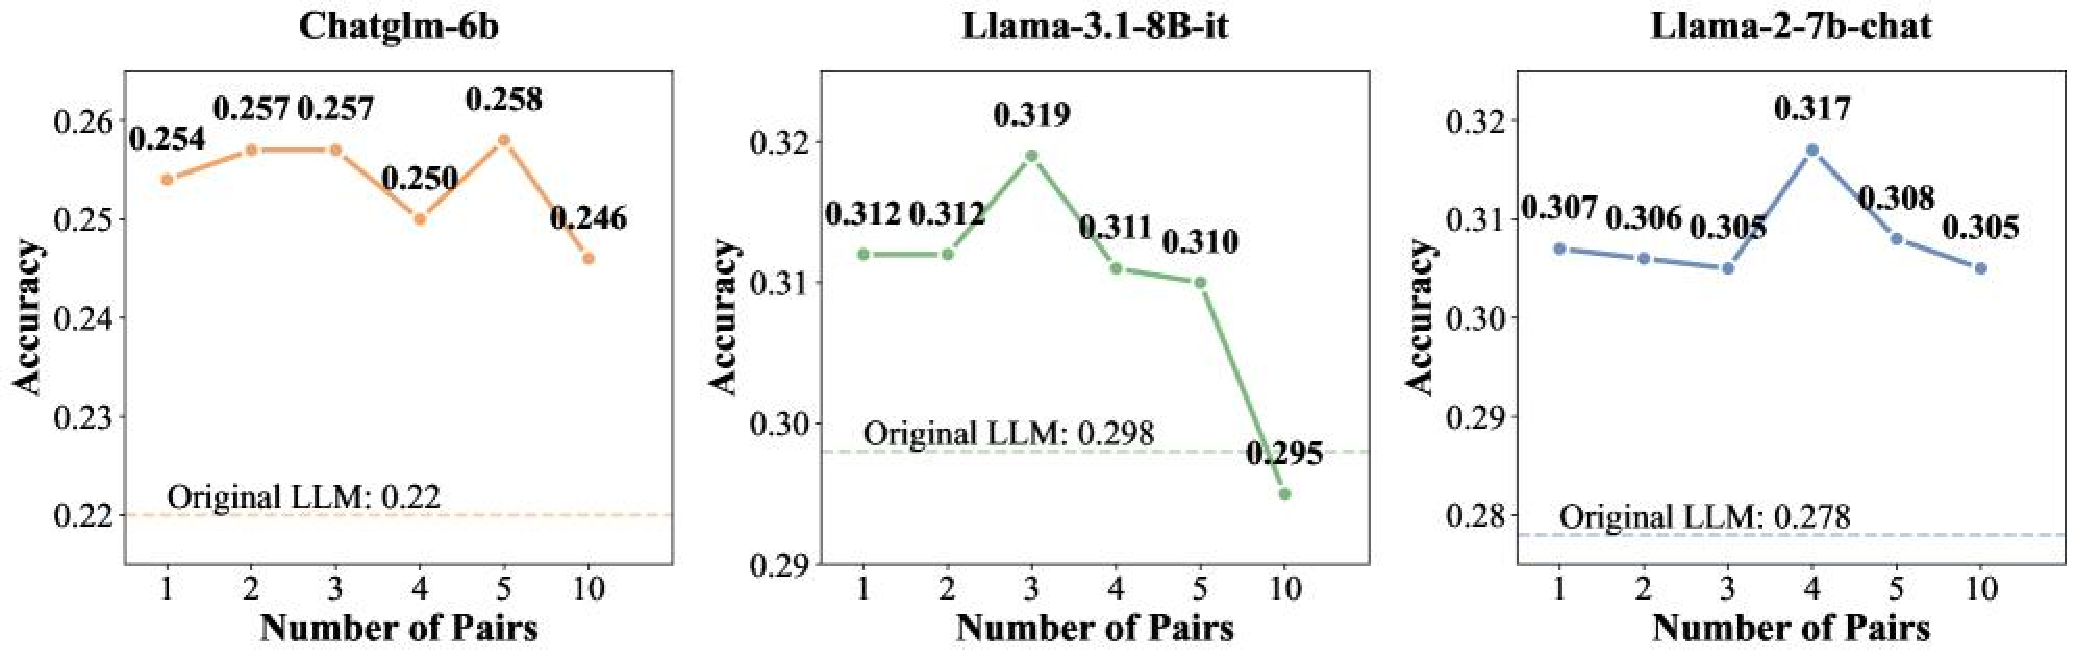
\includegraphics[width=0.95\linewidth]{figures/pairs_analysis.pdf}
      \caption{Accuracy vs. \# Pairs. 3--5 pairs balance effectiveness and efficiency.}
    \end{figure}
  \end{minipage}

  \end{block}

  \begin{alertblock}{Code \& Contact}

  \centering
  \textbf{GitHub:} \texttt{https://github.com/sunxin000/TTARAG} \qquad \textbf{Email:} \texttt{xin.sun@cripac.ia.ac.cn}

  \end{alertblock}

\end{column}

\separatorcolumn

\end{columns}

\end{frame}

\end{document}
